\chapter{Uitvoering \& resultaten}
\section{Gebruikte technologi\"en}
Alle programmatie wordt uitgevoerd in Python, een dynamische \textit{high-level} programmeertaal. Python is ontwikkeld met het oog op leesbare en kernachtige code. Het is een van de meest gebruikte talen voor het uitvoeren van wetenschappelijke experimenten, mede dankzij de vele krachtige bibliotheken die beschikbaar zijn. In dit onderzoek worden de volgende Python-bibliotheken gebruikt:

\begin{itemize}
	\item NumPy: voegt ondersteuning toe voor grote, multi-dimensionale arrays en matrices samen met een groot assortiment aan wiskundige functies om deze arrays effici\"ent te  manipuleren. Deze bibliotheek is een onderdeel van de SciPy-stack (Scientific Python).
	\item Theano \cite{theano}:  een bibliotheek die toelaat wiskundige expressies te defini\"eren, optimaliseren en evalueren. De twee belangrijkste troeven van Theano zijn de dynamische generatie van c-code en het transparante gebruik van GPU-acceleratie. Expressies worden symbolisch omgezet en gecompileerd voor een snelle en effici\"ente uitvoering. Ook worden ze geoptimaliseerd  voor gebruik van de GPU.  Hiernaast biedt de bibliotheek ook heel wat functies voor machine learning. 
	\item Lasagne \cite{lasagne}: een lightweight bibliotheek voor het bouwen en trainen van neurale netwerken. Het biedt verschillende veelgebruikte kosten-, regularisatie-, activatie- en leerfuncties aan alsook vele soorten \textit{layers}. Zo gebruikt dit werk de \textit{DenseLayer} voor volledig verbonden lagen en de \textit{Conv2DLayer} voor de tweedimensionale convolutie. Deze bibliotheek bouwt verder op functionaliteit van Theano waardoor neurale netwerken gebouwd met Lasagne ook gebruik kunnen maken van GPU-acceleratie.
	\item Scikit-learn: deze bibliotheek biedt heel wat machine learning functionaliteit aan maar hiervan wordt in dit onderzoek geen gebruik gemaakt. Het pakket binnen scikit-learn dat wel gebruikt wordt, is \textit{metrics}. Deze wordt gebruikt voor de evaluatie van het model. Vanuit de voorspelde en ware labels kunnen we via diverse functies de kwaliteit van de classificatie beschouwen. Dit pakket wordt voornamelijk gebruikt voor het berekenen van de precision en recall, en het opstellen van de confusion matrix. Deze termen worden verklaard in Sectie \ref{sec:pr-conf}.
	\item Scikit-image: is een verzameling beeldverwerkingsalgoritmes. Deze bibliotheek wordt gebruikt voor de data-augmentatie.
	
\end{itemize}
\section{Dataset}
De gebruikte dataset is die van de ``ChaLearn Looking at People Challenge 2014'' zoals beschreven in \cite{escalera_chalearn_2014}. Uit deze set wordt de derde track gebruikt: ``gesture recognition''. Deze bevat meer dan 14000 gebaren uit een vocabularium van 20 Italiaanse gebaren. Merk op dat het hier niet gaat om een gebarentaal maar om afzonderlijke gebaren uit de Italiaanse cultuur. De verschillende gebaren en hun benamingen zijn te zien in \ref{fig:gebaren}.
\begin{figure}
	\centering
	%	\def\svgscale{0.85}
	\def\svgwidth{\columnwidth}
	\input{figuren/gebaren.pdf_tex}
	\caption{De Italiaanse gebaren gebruikt in de ``ChaLearn Looking At People Challenge 2014, Track 3: gesture spotting''}
	\label{fig:gebaren}
\end{figure}
\npar De gebaren worden uitgevoerd door 27 gebruikers tegen verschillende achtergronden. Er is variatie op vlak van kleding, lichaamsbouw, belichting, gebaaruitvoering. De beelden zijn opgenomen met behulp van een Kinect camera waardoor er vier datastromen zijn: RGB-beeld, dieptebeeld, gebruikersindex en skeletinformatie (Figuur \ref{fig:chalearn-data}).
\begin{figure}
	\centering
	%	\def\svgscale{0.85}
	\def\svgwidth{\columnwidth}
	\input{figuren/chalearn-data.pdf_tex}
	\caption{De vier datastromen beschikbaar in de ``ChaLearn Looking At People Challenge 2014, Track 3: gesture spotting'' dataset}
	\label{fig:chalearn-data}
\end{figure}
\npar Deze dataset werd ook gebruikt in \cite{lionel} waar deze een aantal voorverwerkingsstappen onderging. Deze voorverwerkte dataset is ter beschikking gesteld van dit onderzoek. De voorverwerking probeert de dataset te optimaliseren voor gebarenherkenning. Eerst en vooral worden er vier nieuwe datastromen gecre\"eerd door het uitsnijden van de linker en rechterhand uit zowel diepte- als RGB-beeld. Ook wordt het bovenlichaam ge\"isoleerd om een deel van de achtergrond weg te werken. In totaal zijn er zo zes datastromen beschikbaar. De dataset bestaat uit 10000 ge\"isoleerde gebaren samen met hun correcte klasselabel. Elk beeld bestaat uit 32 frames en heeft een resolutie van 64x64 pixels.

\npar In dit onderzoek wordt de dataset opgedeeld in 60\% training-, 20\% validatie- en 20\% testset.


\section{Onderzoeksopzet}

De experimenten worden uitgevoerd op computers van het Reservoir Lab aan van de vakgroep Elektronica- en Informatiesystemen (ELIS) van de Universiteit Gent. De gebruikte computers hebben een hexacore processor (Intel Core i7-3930K) met kloksnelheid van 3.2 GHz en een NVIDIA Tesla K40c grafische kaart.

\npar In een eerste fase moet er een convolutioneel neuraal netwerk worden opgezet die een aanvaardbare nauwkeurigheid behaald op de gebruikte dataset. Dit model wordt besproken in sectie \ref{sec:basismodel}. De nauwkeurigheden van dit predictief model getraind op alle klassen met alle voorbeelden wordt vervolgens gebruikt als vergelijkingspunt of \textit{baseline} voor de one-shot learning experimenten.

\npar In de volgende stap zal een model, qua architectuur en hyperparameters gelijkend op het basismodel, getraind worden op een deelverzameling van de gebaren. Na deze pre-training kan het model een gebaar bijgeleerd worden en wordt er ge\"experimenteerd met het aantal verschillende samples van het nieuwe gebaar, het aantal lagen dat hertraind worden en met het gebruik van data-augmentatie. De bespreking van deze experimenten gebeurt in sectie \ref{sec:experimenten}.

\section{Basismodel}\label{sec:basismodel}
Alle keuzes omtrent hyperparameters en architectuur zijn experimenteel, op basis van gelijkaardige onderzoeken en naar advies van de begeleiding bepaald. Er zijn vele mogelijke combinaties qua hyperparameters en het is zeer tijdrovend om hierin de meest optimale keuze te maken. Dit is ook niet de essentie van dit onderzoek. Er dient een voldoende goed model opgesteld te worden om vergelijkingen te maken tussen het leren van alle gebaren (basismodel) en het bijleren van een gebaar. 
\subsection{Invoer}
Het beeld van elk gebaar is 64x64 pixels groot en bestaat uit 32 frames. Hieruit worden er 4 frames met volgende indices geselecteerd: 7,13,18 en 25. Er is gekozen om niet van alle input gebruik te maken om een snellere trainingstijd te bekomen zodat er meer experimenten kunenn worden uitgevoerd. In een latere fase of bij verder onderzoek kan het model steeds uitgebreid worden om meer gebruik te maken van spatio-temporele data.
\npar Er wordt enkel gebruik gemaakt van het dieptebeeld, volgens \cite{lionel} en \cite{wu_deep_2014} ligt hierin de nuttigste informatie voor een CNN. Het gebruik van RGB-beeld in combinatie met grijswaardenbeeld voegt meestal weinig toe. Hierin kan dus ook weer rekentijd worden gespaard.
\begin{figure}
	\centering
	%	\def\svgscale{0.85}
	\def\svgwidth{0.5\columnwidth}
	\input{figuren/dataset-input.pdf_tex}
	\caption{De 12 frames gebruikt voor de invoer van het CNN. De frames hebben een resolutie van 64x64 pixels.}
	\label{fig:dataset-input}
\end{figure}
\npar Per voorbeeld zijn er 12 beelden zoals weergegeven in Figuur \ref{fig:dataset-input}. De input van de invoerlaag heeft dus een dimensie van 12x64x64. Merk op dat de beelden van de handen en het volledige bovenlichaam in hetzelfde CNN worden verwerkt. Alle uitgevoerde experimenten hanteren deze invoerdimensie.

\subsection{Architectuur}
\begin{figure}
	\centering
	%	\def\svgscale{0.85}
	\def\svgwidth{\columnwidth}
	\input{figuren/First-model.pdf_tex}
	\caption{Het basismodel bestaande uit een drielagig CNN voor feature-extractie en een drielagig ANN (met softmax uitvoerlaag) voor classificatie}
	\label{fig:model-1}
\end{figure}
Het opgestelde basismodel is weergegeven in figuur \ref{fig:model-1}
Het CNN bestaat uit drie convolutionele en max-pooling lagen. Alle max-pooling gebeurt met vensters van 2x2 zodat het beeld telkens gehalveerd wordt in grootte. De eerste convolutionele laag bevat 8 5x5 filters, de tweede 16 5x5 filters en de laatste 32 4x4 filters.
\npar De output van dit CNN wordt gebruikt als featurevector in een ANN voor classificatie. Het ANN bevat ook drie lagen, de twee verborgen lagen hebben respectievelijk 800 en 100 knopen. Alle verborgen knopen zijn ReLU's en aan de uitgangslaag wordt een softmax gebruikt met 20 units voor de classificatie van de verschillende gebaren.
\begin{table}
	\centering
	%	\vspace{5pt}
	\renewcommand{\arraystretch}{0.8}% 
	\begin{tabular}{ l l }
		\hline
		\textit{Hyperparameter} & \textit{Waarde} \\
		\hline
		\hline
		\textbf{Filters CNN:} & \\
		\quad Laag 1 & 8x(5x5) \\
		\quad Laag 2 & 16x(5x5) \\
		\quad Laag 2 & 32x(4x4) \\
		
		\textbf{Verborgen units ANN:} &\\
		\quad Laag 1 & 800\\
		\quad Laag 2 & 100 \\
		\hline
		Max-pooling vensters & 2x2\\
		Learning rate & $10^{-4}$\\
		Batch grootte & 32\\
		Dropout kans & 0.5\\
		Nesterov momentum & 0.9\\
		\hline
		\textbf{Initialisatie:} & \\
		Gewichten CNN & Glorot initialisatie (uit uniforme verdeling $[-a,a]$)\\
		Bias CNN & 0 \\
		Gewichten ANN & Glorot initialisatie (uit uniforme verdeling $[-a,a]$)\\
		Bias ANN & 0 \\
		\hline
		\textbf{Data-augmentatie:} & \\
		Zoom & [83.33,120] \%, uniforme verdeling \\
		Rotatie & [-2,2]$^{\circ}$, uniforme verdeling\\
		2D translatie & [-2,2] pixels, uniforme verdeling
		
	\end{tabular}	
	\caption{Hyperparameters van het basismodel}\label{tab:hyperparam}
\end{table}
\npar Een samenvatting van alle hyperparameters en gekozen architectuur is te vinden in Tabel \ref{tab:hyperparam}. Voor de regularisatie wordt er gebruik gemaakt van dropout. De gewichten worden ge\"initiaseerd met Glorot gewichten gesampled uit een uniforme verdeling. Deze gewichtsinitialisatie beschreven in \cite{glorot-1} is ontwikkeld voor deep learning methodes en zorgt ervoor dat het signaal tot diep in het netwerk kan reiken. Het is de standaard initialisatie methode van het Lasagne framework.
\npar Er wordt ook aan data-augmentatie gedaan om de prestatie van het predictief model te verbeteren. De parameters van deze augmentatie staan beschreven in Tabel \ref{tab:hyperparam}. Deze parameters bleken later nogal conservatief gekozen, in Sectie \ref{sec:softmax19x1} wordt hierover uitgebreid.
%De gebruikte data-augmentatie bleek bij nader inzien geen zo'n grote impact te hebben door conservatief gekozen parameters zoals weergegeven onderaan Tabel \ref{tab:hyperparam}. De parameters voor translatie en rotatie zijn eigenlijk te klein en voegen weinig variatie toe aan de beelden. In Sectie \ref{sec:model-19x1} wordt hierover verder uitgebreid.
\subsection{Training}
\npar Mini-batch gradient descent aangevuld met Nesterov Augmented Momentum worden gebruikt als optimalisatie-algoritme. Alle training wordt uitgevoerd op de GPU waardoor we de CPU kunnen gebruiken om de voorbeelden aan te voeren. Dit verloopt als volgt:
\begin{itemize}
	\item een werk-proces selecteert 32 random gekozen klasselabels
	\item per gekozen klasselabel wordt een random voorbeeld van die klasse gekozen uit de trainingset
	\item elk voorbeeld wordt geaugmenteerd met behulp van een transformatiematrix
	\item de voorbeelden worden in een array in het gedeelde geheugen geplaatst en opgehaald voor training van het model
	\item tijdens de training op deze mini-batch wordt de volgende klaargezet
\end{itemize}
Na 250 iteraties, die we verder een epoch zullen noemen, wordt het model ge\"evalueerd met de validatieset. Het minimum van de validatiefout wordt bijgehouden en telkens we een lagere waarde bereiken worden de modelparameters opgeslaan. De training stopt wanneer er na een aantal epochs geen verbetering meer te zien is in de validatiefout.

\subsection{Baseline resultaten}
Om de baseline op te stellen wordt de volledige trainingset gebruikt om de 20 gebaren van de dataset te leren classificeren. Het voorgestelde model convergeert na ongeveer 250 epochs en behaalt een totale nauwkeurigheid van 81,20 \%.

\subsubsection{Precision, recall en confusion}\label{sec:pr-conf}
\begin{figure}
	\centering
	%	\def\svgscale{0.85}
	\def\svgwidth{0.7\columnwidth}
	\input{figuren/prec+recall.pdf_tex}
	\caption{Visualisatie van de betekenis van precision en recall. Links zijn alle relevante elementen te zien die zouden moeten geselecteerd worden. Het omcirkelde gedeelte zijn de effectief geselecteerde elementen of de voorspellingen van het model}
	\label{fig:prec+recall}
\end{figure}

\npar In Figuur \ref{fig:conf-allegebaren} is de genormaliseerde confusion matrix van het basismodel te zien. De mate van verwarring valt best mee, voor alle klassen ligt de waarde op de diagonaal relatief hoog. Een aantal klassen worden wel vaak verward zoals bijvoorbeeld klasse 3 en 9 ($\sim$15 \% van klasse 3 en $\sim$20 \% van klasse 9). Ook klasse 13 en 14 worden ondanks hun relatief hoge ware voorspellingswaarde ook vaak verward ($\sim$7 \% van klasse 13 en $\sim$13 \% van klasse 14)

\begin{figure}
	\centering
	\def\svgwidth{0.9\columnwidth}
	\input{figuren/conf_alle_klassen.pdf_tex}
	\caption{Genormaliseerde confusion matrix van baseline voorspellingen van het basismodel, getraind op alle voorbeelden van alle gebaren }
	\label{fig:conf-allegebaren}
	
	\vspace{1cm}
	\begin{tabular}{l l}
		\begin{tabular}{l l l}
			\hline
			\textbf{Label} & \textbf{Precision} &
			\textbf{Recall}\\
			\hline
			0 & 84,71 \% & 77,42 \% \\
			1 & 71,17 \% & 77,45 \% \\
			2 & 81,82 \% & 80,00 \% \\
			3 & 62,04 \% & 67,00 \% \\
			4 & 92,15 \% & 93,07 \% \\
			5 & 87,04 \% & 90,38 \% \\
			6 & 84,71 \% & 77,42 \% \\
			7 & 74,59 \% & 85,05 \% \\
			8 & 93,46 \% & 93,46 \% \\
			9 & 58,54 \% & 49,48 \% \\
			\hline
		\end{tabular} & 
		\begin{tabular}{l l l}
			\hline
			\textbf{Label} & \textbf{Precision} &
			\textbf{Recall}\\
			\hline
			10 & 77,27 \% & 67,33 \% \\
			11 & 84,33 \% & 69,31 \% \\
			12 & 91,57 \% & 92,55 \% \\
			13 & 80,39 \% & 79,61 \% \\
			14 & 56,41 \% & 74,16 \% \\
			\textbf{15} & \textbf{96,88} \% & \textbf{94,90} \% \\
			16 & 91,35 \% & 92,23 \% \\
			17 & 75,27 \% & 72,92 \% \\
			18 & 90,69 \% & 83,87 \% \\
			19 & 91,51 \% & 93,27 \% \\
			\hline
		\end{tabular}	
	\end{tabular}
	\captionof{table}{Precision en recall voor de voorspellingen van het basismodel getraind op alle voorbeelden van alle gebaren.}
	\label{tab:pr-alle-klassen}
\end{figure}

\npar In Tabel \ref{tab:pr-alle-klassen} zijn alle precision en recall scores van het basismodel opgelijst. Deze scores zullen gebruikt worden als baseline voor de experimenten met het bijleren en one-shotten van een gebaar. Het zijn de waardes die we nastreven bij het hertrainen.



\section{Een gebaar bijleren}\label{sec:experimenten}

\subsection{Softmax20 model}\label{sec:softmax20}

De eerste experimenten rond het bijleren van een gebaar worden uitgevoerd op een model volledig gelijk aan het basismodel (zoals afgebeeld in Figuur \ref{fig:model-1}). Eerst wordt het model getraind met een trainingset van 19 gebaren. Als het model geconvergeerd en genoeg geregulariseerd is, zou het een aantal algemene features van een nieuw gebaar moeten herkennen.

\npar De pretraining gebeurt op een softmax van 20 units, een unit wordt dus niet gebruikt. Deze opstelling is niet bruikbaar om een dynamisch uitbreidbaar herkenningssysteem te maken omdat ze ervan uit gaat dat er slechts een gebaar zal worden toegevoegd. Het is wel een goede eerste test van het potenti\"eel van het model.

\npar Door het model te hertrainen met de trainset van 19 gebaren aangevuld met een aantal samples van het nieuwe gebaar leren we het model ook op deze klasse te activeren. Om de hyperparameters van het model te optimaliseren wordt het na elke epoch ge\"evalueerd met de volledige validatieset. Deze bevat alle beschikbare voorbeelden van het nieuwe gebaar zodat er kan gelet worden op overfitting van het model op het kleine aantal trainingsvoorbeelden.

\npar Een finale evaluatie wordt gemaakt met alle voorbeelden uit de testset. Uit de voorspelling op deze testset worden de precision en recall scores van de klasse berekend en ge\"evalueerd.

\begin{figure}
	\centering
	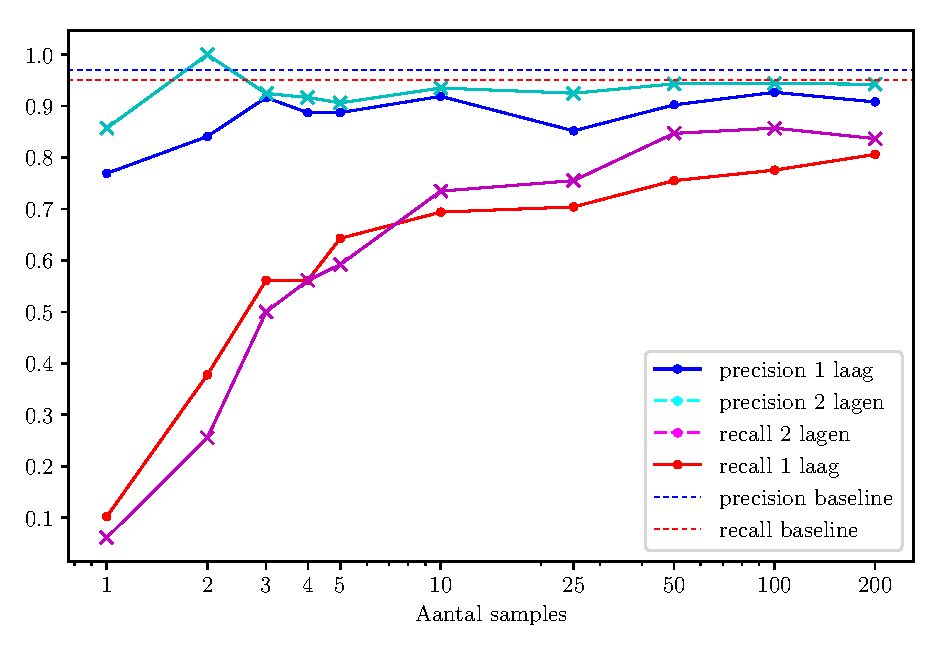
\includegraphics{naive-oneshot-lagen-vergelijking.pdf}
	\caption{Precision en recall voor de classificatie van gebaar 15 met het softmax20 model in functie van het aantal gebruikte samples voor bijleren. De streepjeslijnen geven de baseline weer van het model getrained op alle voorbeelden.}\label{fig:naive-model}
\end{figure}

\npar Eerst en vooral wordt het aantal samples gevari\"eerd. Het model wordt getraind met 200, 100, 50, 25, 10, 5, 4, 3, 2 voorbeelden en ten slotte wordt er 1 voorbeeld gebruikt voor een poging tot one-shot learning.
\npar Ook wordt het effect van het aantal hertrainde lagen onderzocht. Eerst wordt enkel de laatste laag, de softmax, hertraind. Alle andere parameters van het model blijven dus ongewijzigd. In een tweede experiment worden de softmax en de laatste verborgen laag, deze met 100 units, hertraind.

\npar In figuur \ref{fig:naive-model} zijn de resultaten van deze experimenten met het \textit{softmax20} model te zien. Het bijgeleerde gebaar is het gebaar nummer 15: "non ce ne piu". Het basismodel getraind op alle voorbeelden behaalde een 96.88\% precision en 94.90\% recall score op dit gebaar, de hoogste scores van alle gebaren. Enerzijds zou dit gebaar dus gemakkelijk moeten aan te leren zijn aangezien het heel nauwkeurig voorspeld wordt. Anderzijds kan het model zich niet meer beroepen op de features geleerd uit dit gebaar aangezien ze niet in de pretraining is opgenomen.

\npar Het is opvallend dat de precision scores voor beide experimenten heel dicht liggen bij de baseline. Het model is dus redelijk zeker dat het om het nieuwe gebaar gaat als het dit gebaar herkent. Bij het hertrainen van de twee laatste lagen met twee voorbeelden gaat de precisie zelfs boven die van de baseline.

\npar De recall score volgt niet dezelfde lijn als die van de precision. Hier zien we duidelijk dat de recall bij gebruik van weinig samples heel laag ligt. De stijlste klimming bij het model waar enkel de softmax wordt hertraind zien we tot aan het gebruik van 5 samples. Bij het hertrainen van twee lagen loopt deze stijging door tot 10 samples. Dit kan verklaard worden doordat er meer parameters geoptimaliseerd moeten worden bij het het hertrainen van de twee lagen. Meer parameters vragen om meer voorbeelden, bij gebruik van meer dan 10 samples scoort dit model dan  ook beter.

\npar Het voorgetrainde model, GARBAGE CLASS

%\npar Het opzet van dit onderzoek is zo weinig mogelijk samples te gebruiken, voor verdere experimenten werd er dus gekozen om enkel de softmax te hertrainen van het nieuwe gebaar

\subsection{Softmax19+1 model}\label{sec:softmax19x1}
We willen naar een dynamisch uitbreidbaar systeem toewerken. Het vorige model gaat uit van slechts een bij te leren gebaar en is hier dus niet bruikbaar voor. Om aan deze uitbreidbaarheid te voldoen en om verder onderzoek te voeren wordt het \textit{Softmax19+1} model opgesteld, te zien in Figuur \ref{fig:19+1model}.

%FIGUUR

\npar Hier wordt eerst een model met 19 softmax units getraind voor de classificatie van 19 gebaren. Behalve het verschil in aantal softmax units is de architectuur volledig gelijk aan die van het basismodel. Daarna wordt het model uitgebreid met een extra unit voor de classificatie van het nieuwe gebaar. De softmax activatiefunctie van de laag met 19 eenheden wordt vervangen door een lineaire activatie ($a(x)=x$). De signalen van deze units worden samengebracht met het signaal van de nieuwe unit, ook met een lineaire activatiefunctie, in een \textit{ConcatLayer}.  Op deze laatste laag, die nu 20 eenheden telt, wordt dan de softmax uitgevoerd voor classificatie.

\begin{figure}
	\centering
	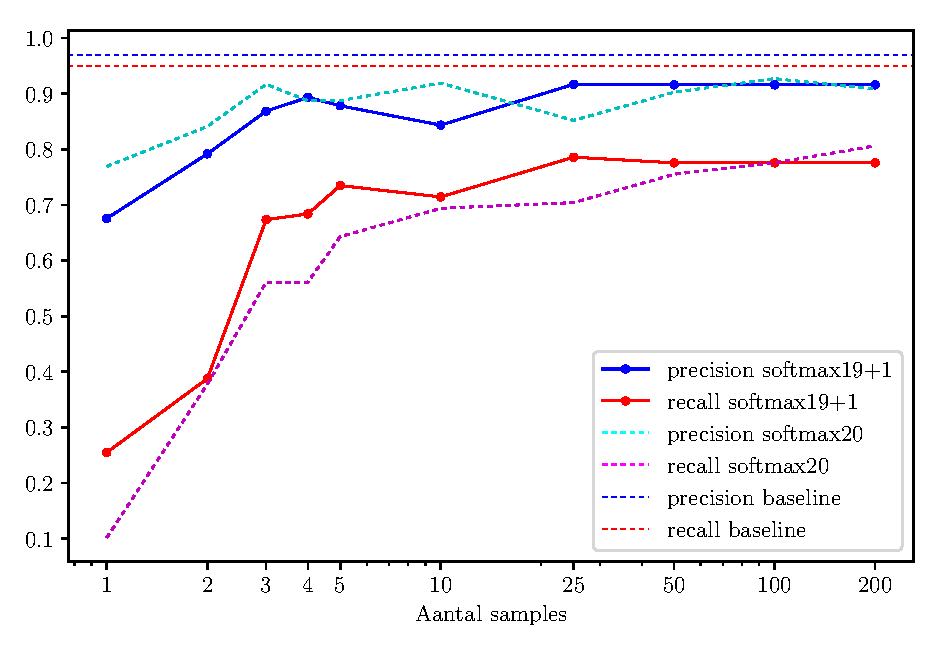
\includegraphics[width=\columnwidth]{19x1-gebaar15.pdf}
	\caption{Precision en recall voor de classificatie van gebaar 15 met het softmax19+1 model in functie van het aantal gebruikte samples voor bijleren.}\label{fig:19x1-gebaar15}
	
		\vspace{0.5cm}
		\def\svgwidth{1.1\columnwidth}
		\input{figuren/19x1-oneshot-vgl.pdf_tex}
		\caption{Barplots per gebaar van de precision en recall van de baseline en na het hertrainen met respectievelijk 1 en 10 samples. }\label{fig:19x1-all}
\end{figure}

\npar Het leren gebeurt enkel op de ene unit van het nieuwe gebaar. Aan de verborgen laag van de 19 al geleerde gebaren wordt niet geraakt zodat het herkenningsvermogen op deze gebaren gelijk blijft. Dit zal ook een vereiste zijn van een uitbreidbaar herkenningssysteem, het bijleren van een nieuw gebaar mag geen negatief effect hebben op de huidige prestatie van het model.

\subsubsection{Invloed van het aantal samples}

Het softmax19+1 model wordt getoetst tegen de prestatie van het softmax20 model. In Figuur \ref{fig:19x1-gebaar15} is de precision en recall van de classificatie van gebaar 15 te zien in functie van het aantal samples dat gebruikt wordt in de trainingset. Ook de prestatie van het softmax20 model bij hertrainen van enkel de softmax laag is geplot in streepjeslijnen. De waarden liggen niet zo heel ver uiteen. De precision van het softmax19+1 model ligt iets lager bij gebruik van minder dan 10 samples. Wel ligt de recall score globaal hoger dan die van het softmax20 model. Bij het trainen op een voorbeeld is dit 25,51 \% tegenover 10,20\%. De recall curve volgt dezelfde stijle klim tot aan het gebruik van 5 samples, tot 73,47\% waarna het nog licht stijgt bij 25 samples en dan rond de 78\% blijft.

\subsubsection{Invloed van het bijgeleerde gebaar}

De prestatie van het softmax19+1 model volgt dus dezelfde trend als die van het softmax20 model. De resultaten hier weergegeven zijn allemaal na het bijleren van gebaar 15. Welk gebaar er bijgeleerd wordt heeft uiteraard ook een invloed op de prestatie van het model. Sommige gebaren hebben vele features gemeenschappelijk met andere gebaren, andere zijn eerder uniek en zullen moeilijk herkend worden.

\npar Om een beeld te scheppen van de invloed van het bij te leren gebaar werd voor elk gebaar eerst een model getraind exclusief dit gebaar, waarna het werd bijgeleerd met 1 en met 10 samples. Op Figuur \ref{fig:19x1-all} zijn de resultaten van dit experiment te zien. Bovenaan is de precision uitgeplot van alle gebaren, onderaan de recall.

\npar De recall score na bijleren met 1 en met 10 samples volgt dezelfde lijn als die van de baseline. Gebaren die een lagere recall score hebben na trainen op alle voorbeelden van alle gebaren scoren ook lager als we ze bijleren. Hetzelfde geldt voor gebaren die hoog scoren. Zeker bij vergelijking van het gebruik van 10 samples is dit opmerkelijk.

\npar De precision volgt ook dezelfde trend maar de verschillen zijn veel kleiner. De bevindingen uit het eerste experiment op gebaar 15 zijn dus door te trekken naar de andere gebaren.

\subsubsection{Invloed van data-augmentatie}
Ten slotte wordt ook nog een experiment opgezet om de invloed van data-augmentatie te onderzoeken. Tot voor dit experiment werd data-augmentatie toegepast met de parameters beschreven in Tabel \ref{tab:hyperparam}. Nieuwe testen worden opgezet die geen augmentatie gebruiken en hier is duidelijk dat de augmentatie weinig tot geen effect heeft. De gekozen parameters blijken erg conservatief en brengen te weinig variatie in de data. Er wordt geprobeerd om een meer drastische data-augmentatie toe te passen. Om met de grotere variatie om te kunnen gaan moet het aantal parameters van het model verhoogd worden. Dit is uitgetest met een model met het dubbele aantal filterbanken in de convolutielagen en twee maal 512 units in de verborgen lagen van het ANN. Na analyse blijkt het model te underfitten: het is nog niet complex genoeg om de geaugmenteerde data te beschrijven. Om deze opstelling te optimaliseren dient er opnieuw een iteratief proces van hyperparameteroptimalisatie aangevat te worden. Hier is niet verder op ingegaan, het gebruik van data-augmentatie kan wel verder onderzocht in toekomstig werk.

\subsection{Softmax18+1+1 model}

Om de uitbreidbaarheid verder te onderzoeken wordt analoog aan het principe van het softmax19+1 model een architectuur gemaakt dat twee gebaren na elkaar bijleert (Figuur \ref{fig:18x2-arch}). Eerst wordt een model met 18 softmax units getraind. Na deze pretraining wordt er een unit voor het bij te leren gebaar toegevoegd en net zoals het vorige model worden de uitgangen van de 18 units en de nieuwe unit samengevoegd met een ConcatLayer.
\npar Het model leert een gebaar bij door de training van het nieuw toegevoegde unit en wordt daarna opnieuw uitgebreid met nog een extra unit voor het tweede gebaar. Ook deze unit wordt geconcateneerd zodat er uiteindelijk een softmax van 20 units is (18+1+1).

\npar Door op deze manier te werk te gaan is het theoretisch mogelijk om gebaren te blijven toevoegen. Na het toevoegen van een aantal gebaren kunnen de units effectief samengevoegd worden tot een laag waarna het proces opnieuw kan beginnen.

\npar In Figuur \ref{fig:18x2} zijn de resultaten te zien van het bijleren van gebaar 13 en gebaar 18. Eerst wordt gebaar 13 bijgeleerd, daarna gebaar 18, telkens met even veel voorbeelden. De recall score van beide gebaren ligt hoger dan wanneer ze elk afzonderlijk worden bijgeleerd in het softmax19+1 model. De precision ligt dan wel weer lager, vooral bij gebaar 13 dat eerst werd aangeleerd.

\npar Waarom de recall hoger ligt dan bij het softmax19x1 model valt moeilijk te verklaren. Het bijleren van een gebaar blijkt in al de experimenten erg afhankelijk van welk gebaar wordt bijgeleerd en uit welke gebaren wordt voorgeleerd. Om dit verder uit te zoeken zouden er meer experimenten met andere gebaren moeten worden uitgevoerd.

\npar Figuur \ref{fig:conf-18x2} geeft de genormaliseerde confusion matrix weer van het bijleren uit een voorbeeld. Hierop is te zien dat er een kleine verwarring is tussen de twee nieuw aangeleerde gebaren: 6\% van gebaar 18 wordt verward met 13 en omgekeerd 3\%. De grootste verwarring bij gebaar 18 is met gebaar 14: 31\%. In het baseline model is dit ook de grootste mate van verwarring bij gebaar 18 (6\%, te zien in Figuur \ref{fig:conf-allegebaren}).


\begin{figure}
	\centering
	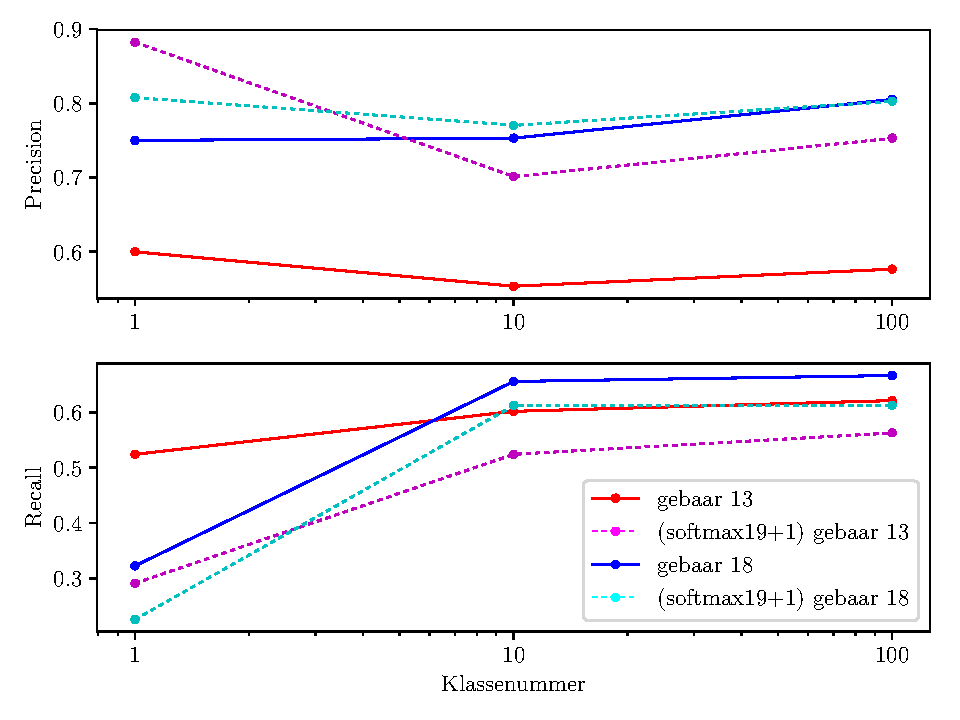
\includegraphics[width=0.90\columnwidth]{18x2.pdf}
	\caption{Precision en recall na het bijleren van gebaar 13 en gebaar 18 in het \textit{softmax18+1+1} model. Ter vergelijking is het resultaat van het \textit{softmax19+1} model ook uitgetekend.}\label{fig:18x2}
	\vspace{1.5cm}
	\def\svgwidth{0.7\columnwidth}
	\input{figuren/conf-18x2.pdf_tex}
	\caption{Genormaliseerde confusion matrix van het \textit{softmax18+1+1} model na leren van gebaar 13 en gebaar 18 met een voorbeeld.}\label{fig:conf-18x2}
\end{figure}